\section{Experimental Evaluation}\label{sec:eval}

\begin{figure}[t]
\small
 \centering\begin{tabular}{|c|c|c|} 
\hline
\multirow{2}{*}{\parbox{2cm}{\centering Scheme}} & \multirow{2}{*}{\parbox{2cm}{\centering Size(GB) for $|DB|=2^{23}$}} & \multirow{2}{*}{\parbox{2cm}{\centering Size(GB) for $|DB|=2^{26}$}} \\ & & \\
\hline 
 \LSDd[\NlogN] & 49 & 436 \\
 \LSDd[\OneChoice] & 7.5 & 60\\
 \SDd[\PiBas] & 5 & 40 \\
\hline
\end{tabular}
%\end{adjustbox}
\caption{Needed storage for a dataset and encrypted index.}
\label{table:storage}
\end{figure} 
%\tgreen{ I/O matters for in memory too.}
%\tgreen{ Repository link of the code}
%\tgreen{why SDd[Pibas] better that SDa[PiBas] in some cases}.
We report the performance of our schemes and compare them with previous state-of-the-art works. 
\begin{figure*}[ht]
	\centering
	\begin{minipage}[t]{0.24\linewidth}
		\includegraphics[width=\textwidth]{chapters/iodse/figures/Search-Comp-DBSize10M-ResultSizeVar-32B-NoCache.eps}
		\vspace{-0.8cm}
		\caption{}
	\end{minipage}
 	\begin{minipage}[t]{0.24\linewidth}
		\includegraphics[width=\textwidth]{chapters/iodse/figures/Search-Comp-DBSize10M-ResultSizeVar-32B-NoCache-SSD.eps}
		\vspace{-0.8cm}
		\caption{}
	\end{minipage}
		\begin{minipage}[t]{0.24\linewidth}
		\includegraphics[width=\textwidth]{chapters/iodse/figures/Search-Comp-DBSizeVar-ResultSize1000.eps}
		\vspace{-.8cm}
		\caption{}
	\end{minipage}
 	\begin{minipage}[t]{0.24\linewidth}
		\includegraphics[width=\textwidth]{chapters/iodse/figures/Search-Comp-DBSizeVar-ResultSize1000-SSD.eps}
		\vspace{-.8cm}
		\caption{}
	\end{minipage}%

	\vspace{-.3cm}
	\caption{Search computation time for $|{DB}|=2^{23}$ and variable result size for (a) $|block|=32$B in (a) HDD, (b) SSD. Search computation time for variable database size and $nw=1K$ in (c) HDD, (d) SSD.}
	\label{fig:search-var}
	%\vspace{-.5em}
\end{figure*}

\begin{figure*}[ht]
	\centering
	\begin{minipage}[t]{0.24\linewidth}
		\includegraphics[width=\textwidth]{chapters/iodse/figures/Search-Comp-DBSize10M-ResultSizeVar-512B-NoCache.eps}
		\vspace{-.8cm}
		\caption{}
	\end{minipage}%
 	\begin{minipage}[t]{0.24\linewidth}
		\includegraphics[width=\textwidth]{chapters/iodse/figures/Search-Comp-DBSizeVar-ResultSize10000.eps}
		\vspace{-.8cm}
		\caption{}
	\end{minipage}~
		\begin{minipage}[t]{0.24\linewidth}
		\includegraphics[width=\textwidth]{chapters/iodse/figures/Search-Comp-DBSizeVar-ResultSize10000-SSD.eps}
		\vspace{-.8cm}
		\caption{}
	\end{minipage}~
  \begin{minipage}[t]{0.24\linewidth}
		\includegraphics[width=\textwidth]{chapters/iodse/figures/SearchTime-WAN2.eps}
		\vspace{-0.6cm}
	\end{minipage}\\
	%\vspace{-.3cm}
	\caption{Search computation time for $|{DB}|=2^{23}$ and variable result size for (a)  $|block|=512$B in HDD. Search computation time for variable database size and $nw=10K$ in (b) HDD, (c) SSD. (d) Search computation time for $|{DB}|=2^{23}$, $|block|=32$B in HDD and variable result size for WAN machines with 24.7ms network delay and 2.5Gbps bandwidth.}
	\label{app-fig:search-var2}
% 	\vspace{-.3cm}
\end{figure*}

We implemented \SDa[\OneChoice], \SDa[\TwoChoice], \SDa[\NlogN], \SDa[\textsf{\Ns}], \LSDd[\OneChoice] and \LSDd[\sN] with approximately 
$31K$ lines in C++. 
We used  OpenSSL-AES~\cite{openssl} 
PRF evaluation and semantically secure encryption. 
We also used Oblivious MAP of~\cite{SDa} {for the \SDd[\PiBas] implementation}, 
and merge-sort as the last step in the implementation of 
bucket oblivious sort~\cite{bucketSort}. We ran our experiments on a machine with
%\tgreen{highlight single core implementation} 
Intel Xeon E-2174G 3.8GHz processor,  128GB  RAM, 1TB SSD, and 5TB HDD running 
Ubuntu 20.04 LTS (limited to one CPU core for our experiments). 
%All schemes were instantiated on a single machine, \tpurp{although communication time between a client and a server can be easily simulated}. 
Our code is available online.\footnote{https://github.com/jgharehchamani/DSE-with-IO-Locality} %\tgreen{SSD/HDD speeds/ RAM speed DDRx ?}







\begin{figure*}[ht]
	\centering
	\begin{minipage}[t]{0.24\linewidth}
		\includegraphics[width=\textwidth]{chapters/iodse/figures/Search-Comp-DBSize10M-ResultSizeVar-32B-NoCache-2.eps}
		\vspace{-0.8cm}
		\caption{}
	\end{minipage}
	\begin{minipage}[t]{0.24\linewidth}
		\includegraphics[width=\textwidth]{chapters/iodse/figures/Search-Comp-DBSize10M-ResultSizeVar-512B-NoCache-2.eps}
		\vspace{-.8cm}
		\caption{}
	\end{minipage}%
		\begin{minipage}[t]{0.24\linewidth}
		\includegraphics[width=\textwidth]{chapters/iodse/figures/Search-Comp-DBSizeVar-ResultSize1000-2.eps}
		\vspace{-.8cm}
		\caption{}
	\end{minipage}~
 	\begin{minipage}[t]{0.24\linewidth}
		\includegraphics[width=\textwidth]{chapters/iodse/figures/Search-Comp-DBSizeVar-ResultSize10000-2.eps}
		\vspace{-.8cm}
		\caption{}
	\end{minipage}~\\
% 	\vspace{-.4cm}
% 	\caption{Search computation time for $|{DB}|=2^{23}$ and variable result size for: (a) $|block|=32$B in HDD, (a) $|block|=32$B in SSD, (c) $|block|=512$B in HDD.}
% 	\label{fig:search-var-block}
	\vspace{-.2cm}
% \end{figure*}

% \begin{figure*}[ht]
% 	\centering
	\begin{minipage}[t]{0.24\linewidth}
		\includegraphics[width=\textwidth]{chapters/iodse/figures/Search-Comp-DBSize10M-ResultSizeVar-32B-NoCache-SSD-2.eps}
		\vspace{-0.8cm}
		\caption{}
	\end{minipage}
	\begin{minipage}[t]{0.24\linewidth}
		\includegraphics[width=\textwidth]{chapters/iodse/figures/Search-Comp-DBSizeVar-ResultSize1000-SSD-2.eps}
		\vspace{-.8cm}
		\caption{}
	\end{minipage}%
		\begin{minipage}[t]{0.24\linewidth}
		\includegraphics[width=\textwidth]{chapters/iodse/figures/Search-Comp-DBSizeVar-ResultSize10000-SSD-2.eps}
		\vspace{-.8cm}
		\caption{}
	\end{minipage}~
	\vspace{-.3cm}
	\caption{Search computation time for $|{DB}|=2^{23}$ and variable result size for (a) $|block|=32$B in HDD, (b) $|block|=512$B in HDD. Search computation time for variable database size and (c) $nw=1K$ in HDD, (d) $nw=10K$ in HDD. Search computation time for $|{DB}|=2^{23}$ and variable result size for (e) $|block|=32$B in SSD. Search computation time for variable database size and (f) $nw=1K$ in SSD, (g) $nw=10K$ in SSD.}
	\label{app-fig:search-var}
% 	\vspace{-.3cm}
\end{figure*}

\begin{figure}[!ht]
	\centering
	\begin{minipage}[t]{0.49\linewidth}
		\includegraphics[width=\textwidth]{chapters/iodse/figures/Search-SDA.eps}
		\vspace{-0.8cm}
		\caption{}
	\end{minipage}
	\begin{minipage}[t]{0.49\linewidth}
		\includegraphics[width=\textwidth]{chapters/iodse/figures/Search-SDA-SSD.eps}
		\vspace{-.8cm}
		\caption{}
	\end{minipage}%
	\vspace{-.3cm}
	\caption{Search computation time for $|{DB}|=2^{23}$, variable result size, and $|block|=32$B for different \NlogN settings in (a) amortized HDD, (b) amortized SSD.}
	\label{app-fig:search-var-amor-deamor}
% 	\vspace{-.3cm}
\end{figure}


We focus on the computation time for Search and Update queries and measure these parameters for variable-size synthetic datasets with $|{DB}| = 2^{11}$-$2^{26}$ records randomly shuffled before insertion, each time setting the total number of distinct keywords $|W|$ to $|{DB}|/100$. Likewise, we report results for varying result size $n_w$ between $10$ and $5M$ documents. We also consider two block sizes: 32B and 512B. %\tgreen{why this two blocksize only} 
%To demonstrate the importance of I/O in environment with limited available memory, we perform the experiments in a cold cache environment. 
\neww{To highlight the significance of I/O in a memory-constrained environment, we conduct our experiments in a cold cache setting, but we also provide two sets of experiments to show the effect of cache on the performance of our schemes. In the first one, we keep the different ratios of datasets in the memory (as cache) and respond to the queries for those encrypted data from memory. Note that we normalize the cache for each scheme. In other words, we fix the cache size and load as much as data we can in that memory.}
% Clearly, schemes with more storage need can benefit less from the cache. 
\neww{In the second, we assume there are many users ($200$ for HDD and $75$ for SSD) each of which has her own dataset with size $2^{20}$ and they execute their own search queries randomly when the cache in the system is enabled.}

Experiments were repeated five times, and the average result is reported. \neww{We also provide a comparison between the needed storage on the server for each de-amortized scheme in Figure~\ref{table:storage} for a dataset with $|block|=32B$ where $|DB|=2^{23}$ and $|DB|=2^{26}$. Note that we focus on small client storage schemes. Therefore, client storage is constant.}


We also repeated the search experiments on a real dataset  consisting of $22$ attributes and $6,123,276$ records of reported crime incidents in Chicago~\cite{crimes}. We used two different attributes, containing 34 and 170 distinct keywords, respectively, and keyword frequency ranging from $1$ record to $1,631,721$ records.
\neww{Finally, we simulated the search and update time of our schemes when run over WAN with 24.7ms delay and 2.5Gbps bandwidth on AWS (between two machines on Ireland and Frankfurt zones).}

\subsection{Search Performance}
Our first set of experiments focuses on search performance and we demonstrate the impact of variable data block sizes, variable result sizes, variable database sizes, \neww{and cache size on all our schemes and compare them with \SDa[\PiBas]~\cite{SDa} and \SDd[\PiBas]~\cite{SDa}. We do not provide the big-block experiments for SSD due to disk space limits.}
%\todo{15. Explain if experimental results can be reproduced in more realistic settings}

\smallskip\noindent\textbf{Variable Block and Result Sizes.} Figure~\ref{fig:search-var} (a,b) and  Figure~\ref{app-fig:search-var2} (a) show the search computation time of a dataset with size $2^{23}$  $|block|=32$B as the result size $n_w$ changes. Similar results for our amortized schemes are in Figure~\ref{app-fig:search-var} (a),(b),(e).

% (results for $|block|=512$B are in Appendices~\ref{append:perf-amort} and~\ref{append:perf-deamort}. 
% a
% nd \ref{}). 
The  conclusions from these experiments are: 
(i) As expected, \SDa[\PiBas] and \SDd[\PiBas]\ have the worst performance among all other schemes for large result sizes due to their poor locality (in HDD) and page efficiency (in SSD). They need to change the position of the hard-drive head or bring different pages of the results, stored at random locations, which leads to significant {slowdown}. (ii) The \SDa[\NlogN]\ and \LSDd[\NlogN] schemes achieve the best performance in the amortized and de-amortized setting, at the cost of extra storage. The number of indexes searched in \LSDd[$\cdot$] is three times than that of \SDa[$\cdot$], hence the search time of \LSDd[\NlogN] is slightly 
more than \SDa[\NlogN]. (iii) \SDa[\TwoChoice] performs better than \SDa[\OneChoice] for small result sizes. However, their performance is the same for result sizes more than the bin's threshold, since, after the threshold entries are stored using \SDa[\OneChoice] (therefore we ignored this scheme in SSD experiments). (iv) The execution time for \SDa[\OneChoice] for result sizes bigger than $10^5$ remains approximately constant, as at this point the database is read in its entirety (i.e. all bins contain results). (v) When the block size is increased from 32B to 512B, 
the search time of all schemes increases, but the gap between \SDa[\TwoChoice]/\SDa[\OneChoice] and \SDa[\PiBas] decreases. This is due to the increase in the volume of the data read for blocks of size 512B, which becomes the dominant factor in the performance. (vi) Amortized and de-amortized versions of \PiBas, \OneChoice, and \NlogN\ have similar performance.
Finally, all our schemes have excellent performance in practice. E.g., \SDa[\OneChoice] and \SDa[\NlogN]/\LSDd[\NlogN] are up to three orders of magnitude faster than \SDa[\PiBas]/\SDd[\PiBas] (for $|n_w|=10^5$ and $|DB|=2^{23}$ \SDa[\OneChoice], \SDa[\NlogN], and \SDa[\PiBas] take 16s, 0.8s, and 903s respectively).


\smallskip\noindent\textbf{Variable Database Size.} Figures~\ref{fig:search-var} (c,d) and Figures~\ref{app-fig:search-var2} (b),(c) show the effect of database size on search computation. (Results for the amortized schemes are in Figures~\ref{app-fig:search-var2} (c),(d),(f),(g)). For small blocks it varies search time for variable database sizes between $2^{11}-2^{26}$ and for result size $n_w$=1K in HDD and SSD. As the figures show, the search time of all schemes increases as the database size increases, because of the added levels in the data structures. However, all our schemes are significantly faster than \SDa[\PiBas] and \SDd[\PiBas]. For instance, the amortized schemes \SDa[\OneChoice], \SDa[\TwoChoice], and \SDa[\NlogN] are faster than \SDa[\PiBas] by $2-136\times$, $5-159\times$, and $4-209\times$ respectively. Also, the de-amortized schemes, \LSDd[\OneChoice] and \LSDd[\NlogN] are faster than \SDd[PiBAS] by $2-58\times$ and $3-70\times$ respectively.

\begin{figure*}[ht]
	\centering
	\begin{minipage}[t]{0.24\linewidth}
		\includegraphics[width=\textwidth]{chapters/iodse/figures/Cache-25.eps}
		\vspace{-.8cm}
		\caption{}
	\end{minipage}%
		\begin{minipage}[t]{0.24\linewidth}
		\includegraphics[width=\textwidth]{chapters/iodse/figures/Cache-50.eps}
		\vspace{-.8cm}
		\caption{}
	\end{minipage}~
 	\begin{minipage}[t]{0.24\linewidth}
		\includegraphics[width=\textwidth]{chapters/iodse/figures/Cache-75.eps}
		\vspace{-.8cm}
		\caption{}
	\end{minipage}
 	\begin{minipage}[t]{0.24\linewidth}
		\includegraphics[width=\textwidth]{chapters/iodse/figures/Cache-100.eps}
		\vspace{-0.8cm}
		\caption{}
	\end{minipage}~\\
	\vspace{-.4cm}
	\caption{Search computation time for $|{DB}|=2^{23}$ and variable result size for $|block|=32$B in HDD, (a) 25\% Caching, (b) 50\% Caching, (c) 75\% Caching, (d) 100\% Caching.}
	\label{fig:cache-hdd}
	%\vspace{-.2cm}
\end{figure*}
\begin{figure*}[ht]
	\centering
	\begin{minipage}[t]{0.24\linewidth}
		\includegraphics[width=\textwidth]{chapters/iodse/figures/Cache-25-SSD.eps}
		\vspace{-.8cm}
		\caption{}
	\end{minipage}%
		\begin{minipage}[t]{0.24\linewidth}
		\includegraphics[width=\textwidth]{chapters/iodse/figures/Cache-50-SSD.eps}
		\vspace{-.8cm}
		\caption{}
	\end{minipage}~
 	\begin{minipage}[t]{0.24\linewidth}
		\includegraphics[width=\textwidth]{chapters/iodse/figures/Cache-75-SSD.eps}
		\vspace{-.8cm}
		\caption{}
	\end{minipage}
    \begin{minipage}[t]{0.24\linewidth}
		\includegraphics[width=\textwidth]{chapters/iodse/figures/Cache-100.eps}
		\vspace{-0.8cm}
		\caption{}
	\end{minipage}~\\
	\vspace{-.4cm}
	\caption{Search computation time for $|{DB}|=2^{23}$ and variable result size for $|block|=32$B in SSD, (a) 25\% Caching, (b) 50\% Caching, (c) 75\% Caching, (d) 100\% Caching.}
	\label{fig:cache-ssd}
	%\vspace{-.2cm}
\end{figure*}

\begin{figure}[ht]
	\centering
	\begin{minipage}[t]{0.48\linewidth}
		\includegraphics[width=\textwidth]{chapters/iodse/figures/email-hdd.eps}
		\vspace{-0.6cm}
		\caption{}
	\end{minipage}
 \begin{minipage}[t]{0.48\linewidth}
		\includegraphics[width=\textwidth]{chapters/iodse/figures/email-ssd.eps}
		\vspace{-0.6cm}
		\caption{}
	\end{minipage}
	\vspace{-.3cm}
	\caption{Search computation time for $|{DB}|=2^{20}$ for each user and variable result size for $|block|=32$B with caching enabled in (a) HDD where 200 users exist in the system (b) SSD where 75 users exist in the system}
	\label{fig:email}
% 	\vspace{-.3cm}
\end{figure}



\smallskip\noindent\textbf{Effect of the value of \emph{s} on \SDa[\NlogN] and \LSDd[\NlogN].} The previous experiments showed that our \NlogN-based schemes have the best performance at a cost 
of more (i.e. $\log N$ times) storage.
% \footnote{For the vanilla \NlogN\ scheme the value of $s$ is $\log N$}. 
However, as discussed in Section ~\ref{sec:obliviousMerge}, these schemes can be used more "cleverly" to reduce the storage overhead. In Figure~\ref{fig:search-var} (a,b), we measured the effect of keeping $s$ intermediate levels instead $\log N$ levels for the de-amortized schemes (e.g., \LSDd[\textsf{3N}] refers to keeping 3 levels).  Similar experiments for amortized schemes are presented in Figure~\ref{app-fig:search-var-amor-deamor}. %We tried to store the entries at an existing level. 
If the level that a keyword-list should be stored does not exist, we split the 
list into multiple equal-sized chunks (last chunk is padded, if necessary) 
and store them in the next closest existing level. The experiment shows that even when keeping fewer levels than $\log N$, \SDa[\NlogN]/\LSDd[\NlogN] outperform \PiBas\ and \OneChoice\ based schemes in terms of search time, due to its practical locality and page efficiency, while also reducing storage to $3s\times N$. E.g., when storing every 8th level (\SDa[\textsf{3N}]/\LSDd[\textsf{3N}]), the achieved scheme is up to $30\times$ and $1949\times$ faster than \SDa[\OneChoice] and \SDa[\PiBas] and up to $8\times$ and $833\times$ faster than {\LSDd[\OneChoice]} and \LSDd[\PiBas] for big result sizes. 


\smallskip\noindent\textbf{Cache Experiment.}
 \neww{Figures~\ref{fig:cache-hdd} and \ref{fig:cache-ssd} show the effect of cache on the search time. They represent the search computation time over a dataset with size $2^{23}$ and $|block|=32B$ for variable result sizes and variable cache sizes on HDD (Figure~\ref{fig:cache-hdd}) and SSD (Figure~\ref{fig:cache-ssd}).
 % in Appendix~\ref{append:perf-deamort}). 
 As explained above, for these experiments we fix the cache size in memory according to the \SDd[\PiBas] scheme which has the smallest storage size in the de-amortized schemes (e.g., $25\%$ of the encrypted dataset of \SDd[\PiBas]), and we use the same cache size as for other schemes for fairness. The figures show that: i) as the cache size increases, all schemes' perform better and their search time reduces. However, \SDd[\PiBas] benefits more from the cache than others (i.e., its search time improves up to 8$\times$ while \LSDd[\OneChoice] and \LSDd[\NlogN] only improve up to $2.4\times$ and $2\times$) due to the smaller needed storage. ii) all our schemes still outperform \SDd[\PiBas] for big enough result sizes ($>$1K). Even when $75\%$ of data is cached in \SDd[\PiBas], \LSDd[\OneChoice] and \LSDd[\NlogN] are up to $191\times$ and $641\times$ faster. iii) When all data is cached (assuming it fits entirely in memory), \LSDd[\NlogN] outperforms other schemes (as expected) because it has the best locality and needs minimal cryptographic operations. On the other hand, \LSDd[\OneChoice] becomes worse than \SDd[\PiBas] in big result sizes because in these queries the dominant overhead comes from crypto and \LSDd[\OneChoice] needs to execute ${\sim}3\times$ more decryptions than the other schemes due to padding.}



\neww{In a second experiment (Fig.~\ref{fig:email})
% in Appendix~\ref{append:perf-deamort}) 
we emulate a scenario with multiple users ($200$ for HDD and $75$ for  SSD) each with her own independent dataset (of size $2^{20}$). With cache enabled, we executed random queries among users. As the figure shows, due to the size of datasets being larger than the memory (encrypted indexes for HDD and SSD were 1.8TB and 675GB), we see a similar trend as Figures~\ref{fig:search-var} (a, b).}


\begin{figure}[t]
	\centering
	\begin{minipage}[t]{0.48\linewidth}
		\includegraphics[width=\textwidth]{chapters/iodse/figures/Search-Crime1.eps}
		\vspace{-0.8cm}
		\caption{}
	\end{minipage}
	\begin{minipage}[t]{0.48\linewidth}
		\includegraphics[width=\textwidth]{chapters/iodse/figures/Search-Crime2-2.pdf}
		\vspace{-.8cm}
		\caption{}
	\end{minipage}%
	
	\vspace{-.3cm}
	\caption{Crime Dataset---Search computation time vs variable result size for an attributed with (a) $|W|=34$, (b) $|W|=170$.}
	\label{app-fig:real}
% 	\vspace{-.3cm}
\end{figure}


\smallskip\noindent\textbf{Search Over Real Datasets.}  We evaluated search times on two attributes of the crime dataset~\cite{crimes}, with (a) $34$, and (b) $170$ distinct keywords. We measured the search time for different keywords associated with increasing numbers of results. Our experiments show that our schemes clearly outperform both \SDa[\PiBas] and \LSDd[\PiBas], and we reach similar conclusions as previously (Figure~\ref{app-fig:real}). 



\smallskip\noindent\textbf{Search Over WAN}
\neww{We also simulated the end-to-end search time when client and server are located on two different machines. Our testbed was two AWS machines in Ireland and Frankfurt (with 24.7ms delay and 2.5Gbps bandwidth). Our experiments show a similar trend as the single machine case due to the constant roundtrip number and high network bandwidth, so our schemes outperform \SDa[\PiBas] and \SDd[\PiBas] (see Fig.~\ref{app-fig:search-var} (d)).}


\subsection{Update Performance}
Next, we report the update performance of our schemes via two sets of experiments: (i) update cost of the amortized scheme, (ii) update cost of the de-amortized schemes.

\smallskip\noindent\textbf{Update Cost of Amortized schemes.} In the first experiment, we measured the update time for 1K consecutive updates. Each time, the client fetches and merges some previously built levels and then uploads them to the server. Clearly, the update cost depends on the number of previously inserted indexes and it increases when more indexes need to be merged. We repeated the same experiment for \SDa[\NlogN] and saw the same behaviour (see Figure~\ref{app-fig:update}). 
%\SDa[\PiBas] has the best update time for small merges and the worst update time for big merges. In this experiment \SDa[\NlogN] varies between 58ms and 6421ms.
It is clear that \SDa[\PiBas] has the best update cost for small merges (due to  storing fewer  entries) and the worst update cost for big merges (as random I/Os increases). The minimum and maximum observed time for \SDa[\PiBas] is $2$ms and $12905$ms, while for \SDa[\NlogN] they are 58ms and 6421ms.



\begin{figure}[!ht]
	\centering
	\begin{minipage}[t]{0.48\linewidth}
		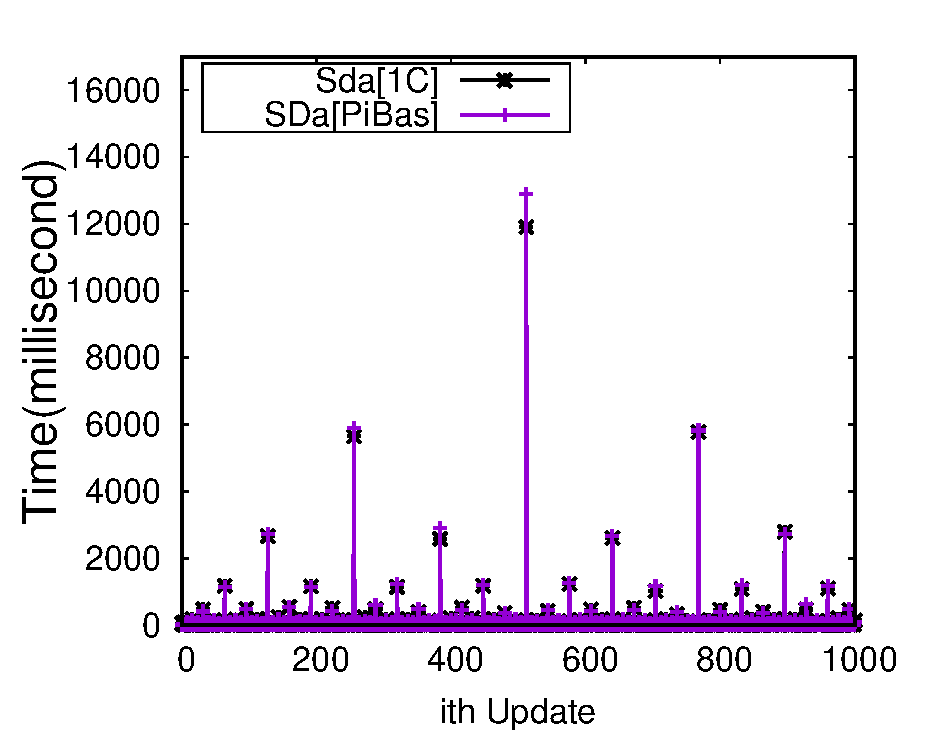
\includegraphics[width=\textwidth]{chapters/iodse/figures/Insert-SDA2.eps}
		\vspace{-0.6cm}
		\caption{}
	\end{minipage}
 \begin{minipage}[t]{0.48\linewidth}
		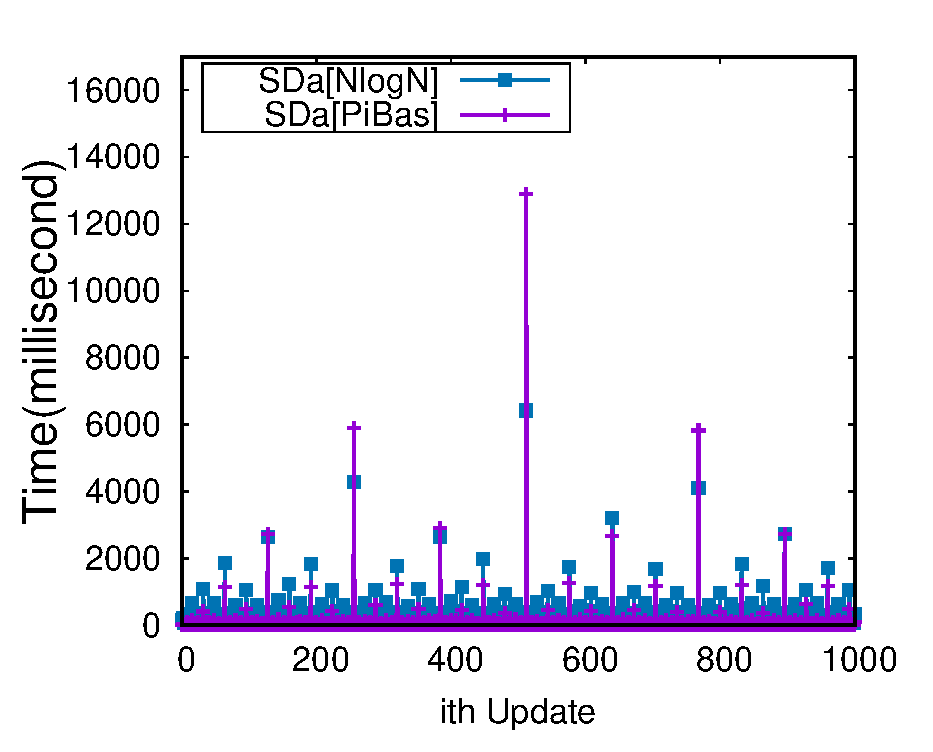
\includegraphics[width=\textwidth]{chapters/iodse/figures/Insert-SDA3.eps}
		\vspace{-0.6cm}
		\caption{}
	\end{minipage}
	\vspace{-.3cm}
	\caption{Update computation time of amortized schemes for 1K updates starting from an empty dataset (a) \SDa[\OneChoice] vs \SDa[\PiBas] (b) \SDa[\NlogN] vs \SDa[\PiBas] }
	\label{app-fig:update}
% 	\vspace{-.3cm}
\end{figure}

\begin{figure}[t]
	\centering
 \begin{minipage}[t]{0.48\linewidth}
		\includegraphics[width=\textwidth]{chapters/iodse/figures/UpdateTime.eps}
		\vspace{-0.6cm}
		\caption{}
	\end{minipage}
 \begin{minipage}[t]{0.48\linewidth}
		\includegraphics[width=\textwidth]{chapters/iodse/figures/UpdateTime-WAN1.eps}
		\vspace{-0.6cm}
		\caption{}
	\end{minipage}
	\vspace{-.3cm}	
	\caption{Update computation time for variable database sizes (a) over single machine (b) over WAN machines with 24.7ms network delay and 2.5Gbps bandwidth.}
	\label{fig:wan}
% 	\vspace{-.3cm}
\end{figure}
	

\smallskip\noindent\textbf{Update Cost of De-Amortized schemes.} To measure the update performance of our de-amortized schemes, first we measured the update computation time for variable database sizes in memory. According to our experiment (Figure~\ref{fig:wan} (a)), \LSDd[\OneChoice] outperforms other schemes for database sizes above $100K$ which is compatible with its better asymptotics (e.g., \LSDd[\OneChoice] is up to {$2.5\times$} faster than \SDd[\PiBas]\ for database size of 5M). Furthermore, \LSDd[\NlogN] has the worst performance in the memory setting due to the large number of layers it needs to create for each level of the de-amortized framework. \neww{We also provided \LSDd[\PiBas] update time to show our framework is applicable to \SDd[\PiBas] and can reduce its cost from $O(\log^3 N)$ to $O(\log^2 N)$.}
Finally, we re-executed this using HDD storage. We observe that \LSDd[\OneChoice] is still the most efficient scheme in all database sizes. On the other hand, \LSDd[\NlogN] becomes better than \SDd[\PiBas] in bigger database sizes due to its better locality (e.g., \LSDd[\OneChoice] and \LSDd[\NlogN] are {$123\times$ and $5\times$} faster than \SDd[\PiBas]\ for size 5M).


\smallskip\noindent\textbf{Update Over WAN.}
\neww{We measured end-to-end update times when client and server are located on different AWS machines, as above (Figure~\ref{fig:wan} (b)). The performance of memory-based \SDd[\PiBas] worsens due to the round trips for OMAP access and the amount of data that must be transferred over the network (\LSDd[\OneChoice] is {$8-11.3\times$} and \LSDd[\NlogN] is {$1.2-2\times$} faster than \SDd[\PiBas]). That said, the performance of disk-based schemes is similar to the single-machine case as the disk overhead is the dominant cost and the bandwidth is high enough to ``cover'' for the network overhead.}





